\documentclass[tikz,border=4pt]{standalone}
\usepackage{tikz}
\usetikzlibrary{calc}
\definecolor{nebula}{HTML}{6366F1}
\definecolor{spark}{HTML}{14B8A6}
\begin{document}
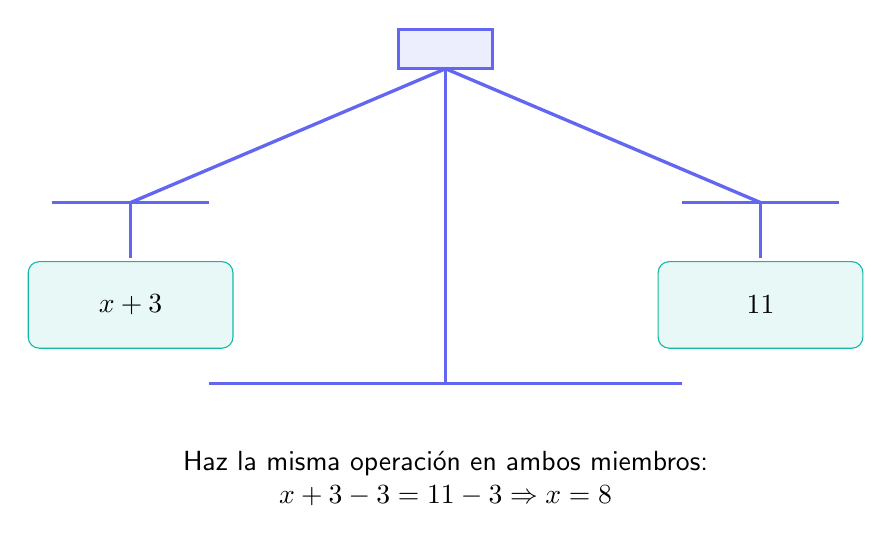
\begin{tikzpicture}[font=\sffamily]
  \draw[very thick,nebula] (0,0)--(0,4);
  \draw[very thick,nebula] (-3,0)--(3,0);
  \draw[fill=nebula!12,draw=nebula,very thick] (-.6,4) rectangle (.6,4.5);
  \draw[very thick,nebula] (0,4)--(-4,2.3) (0,4)--(4,2.3);
  \draw[very thick,nebula] (-5,2.3)--(-3,2.3) (3,2.3)--(5,2.3);
  \draw[very thick,nebula] (-4,2.3)--(-4,1.6) (4,2.3)--(4,1.6);
  \node[rounded corners,draw=spark,fill=spark!10,minimum width=26mm,minimum height=11mm] at (-4,1) {$x+3$};
  \node[rounded corners,draw=spark,fill=spark!10,minimum width=26mm,minimum height=11mm] at (4,1) {$11$};
  \node[align=center] at (0,-1.2) {Haz la misma operaci\'on en ambos miembros:\\$x+3-3=11-3\Rightarrow x=8$};
\end{tikzpicture}
\end{document}
